% ===================================================================
%  Week 4 — Session 1: Noise models & the two core filters
% ===================================================================
\documentclass[10pt,aspectratio=169]{beamer}
% ===================================================================
%  Shared Beamer preamble for "Practical Image Processing"
%  English slides. Compile with pdfLaTeX.
% ===================================================================

\usetheme{metropolis}
\usepackage[T1]{fontenc}
\usepackage[utf8]{inputenc}
\usepackage{lmodern}
\usepackage{listings}
\usepackage{tcolorbox}
\usepackage{fontawesome5}
\usepackage{booktabs}
\usepackage{amsmath,amssymb}
\usepackage{tikz}
\usepackage{pgfplots}
\pgfplotsset{compat=1.17}
\usetikzlibrary{arrows.meta,positioning,shapes.geometric,fit,backgrounds,matrix}
\tcbuselibrary{skins,breakable}

% ---- Palette --------------------------------------------------------
\definecolor{coursePrimary}{HTML}{1B4965}   % deep blue
\definecolor{courseAccent}{HTML}{E76F51}    % coral
\definecolor{courseGood}{HTML}{2A9D8F}      % teal
\definecolor{courseBad}{HTML}{C0392B}       % red
\definecolor{courseInfo}{HTML}{2980B9}      % blue
\definecolor{codeBg}{HTML}{F5F6FA}
\definecolor{codeKw}{HTML}{8E44AD}
\definecolor{codeStr}{HTML}{2A9D8F}
\definecolor{codeCom}{HTML}{7F8C8D}

\setbeamercolor{frametitle}{bg=coursePrimary}
\setbeamercolor{progress bar}{fg=courseAccent}
\setbeamercolor{alerted text}{fg=courseAccent}
\metroset{block=fill,sectionpage=progressbar,numbering=fraction}

% ---- Code listings (Python is built into listings) -----------------
\lstdefinestyle{course}{
  backgroundcolor=\color{codeBg},
  basicstyle=\ttfamily\scriptsize,
  keywordstyle=\color{codeKw}\bfseries,
  stringstyle=\color{codeStr},
  commentstyle=\color{codeCom}\itshape,
  numberstyle=\tiny\color{codeCom},
  numbers=left, numbersep=6pt,
  showstringspaces=false, breaklines=true, breakatwhitespace=true,
  tabsize=4, columns=fullflexible,
  frame=single, framesep=4pt, rulecolor=\color{gray!30},
  keepspaces=true, upquote=true, language=Python,
}
\lstset{style=course}
\lstdefinelanguage{bash}{
  keywords={cd,pip,python,venv,source,import}, sensitive=true,
  morecomment=[l]{\#}, morestring=[b]', morestring=[b]",
}

% ---- Reusable callout boxes ----------------------------------------
\newtcolorbox{goodbox}[1][Good practice]{colback=courseGood!8,colframe=courseGood,
  fonttitle=\bfseries,title={\faCheck~#1},boxrule=0.6pt,left=4pt,right=4pt,top=3pt,bottom=3pt}
\newtcolorbox{badbox}[1][Pitfall]{colback=courseBad!8,colframe=courseBad,
  fonttitle=\bfseries,title={\faTimes~#1},boxrule=0.6pt,left=4pt,right=4pt,top=3pt,bottom=3pt}
\newtcolorbox{infobox}[1][Note]{colback=courseInfo!8,colframe=courseInfo,
  fonttitle=\bfseries,title={\faInfoCircle~#1},boxrule=0.6pt,left=4pt,right=4pt,top=3pt,bottom=3pt}
\newtcolorbox{mathbox}[1][Math]{colback=coursePrimary!6,colframe=coursePrimary,
  fonttitle=\bfseries,title={\faCalculator~#1},boxrule=0.6pt,left=4pt,right=4pt,top=3pt,bottom=3pt}

\newcommand{\keyidea}[1]{\begin{alertblock}{Key idea}#1\end{alertblock}}
\newcommand{\term}[1]{\textbf{\color{coursePrimary}#1}}
\newcommand{\code}[1]{\lstinline[basicstyle=\ttfamily\small]|#1|}

% ---- A helper to draw a small pixel grid, cells shaded by value ----
% \pixelgrid{ {10,20,120,200,240}, {30,60,130,180,230}, ... }
\newcommand{\pixelgrid}[1]{%
  \begin{tikzpicture}[font=\scriptsize,scale=0.6]
    \foreach \row [count=\ry] in {#1} {
      \foreach \val [count=\cx] in \row {
        \draw[gray,fill=coursePrimary!8] (\cx,-\ry) rectangle ++(1,-1);
        \node at (\cx+0.5,-\ry-0.5) {\val};
      }
    }
  \end{tikzpicture}}


\title{Noise \& Restoration}
\subtitle{Week 4 — Session 1: Modelling noise \& the two core filters}
\author{Practical Image Processing}
\date{Lecture 4.1 \textbullet\ 60--70 min}

\begin{document}

\maketitle

\begin{frame}{Recap \& today}
  \begin{columns}[T]
    \begin{column}{0.58\textwidth}
      \begin{itemize}
        \item Wk3: filters combine a pixel with its neighbours (convolution).
        \item \alert{Today:} \term{noise} — where it comes from, how to \term{model} it,
              and the \term{two core filters} (averaging \& median) that cover most cases.
        \item Session 2 will add edge-preserving filters, deblurring, and how to \emph{measure} restoration.
      \end{itemize}
    \end{column}
    \begin{column}{0.42\textwidth}
      \begin{alertblock}{Why it matters}
        Real meter photos are noisy (low light, high ISO). Denoising is what makes the digits
        thresholdable and readable for DocScan.
      \end{alertblock}
    \end{column}
  \end{columns}
\end{frame}

\begin{frame}{Roadmap}\tableofcontents\end{frame}

% ==================================================================
\section{Noise models}
% ==================================================================

\begin{frame}{Two noises you must recognize}
  \begin{columns}[T]
    \begin{column}{0.33\textwidth}\begin{center}
      
\includegraphics[width=\linewidth]{../assets/clean.png}\\{\scriptsize clean}
    \end{center}\end{column}
    \begin{column}{0.33\textwidth}\begin{center}
      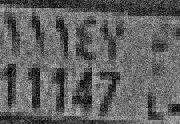
\includegraphics[width=\linewidth]{../assets/gaussian_noise.png}\\{\scriptsize Gaussian}
    \end{center}\end{column}
    \begin{column}{0.33\textwidth}\begin{center}
      
\includegraphics[width=\linewidth]{../assets/sp_noise.png}\\{\scriptsize salt-and-pepper}
    \end{center}\end{column}
  \end{columns}
  \vspace{3pt}
  \keyidea{The noise \emph{type} decides the \emph{cure}. Gaussian $\rightarrow$ averaging; impulse $\rightarrow$ median. Diagnose first.}
\end{frame}

\begin{frame}{Where noise comes from (physics, Week 1)}
  \begin{itemize}
    \item \term{Gaussian noise}: small random fluctuations added to every pixel (sensor/read noise, amplifier noise).
    \item \term{Salt-and-pepper} (impulse): random pixels stuck at 0 or 255 (dead pixels, bit errors in transmission).
    \item \term{Poisson} (shot) noise: from photon counting; stronger in dark areas / low light.
  \end{itemize}
  \begin{mathbox}
    Additive Gaussian model: $g(x,y) = f(x,y) + n(x,y)$, with $n\sim\mathcal{N}(0,\sigma^2)$ — additive, zero-mean, and independent of the signal.
  \end{mathbox}
\end{frame}

\begin{frame}{Poisson (shot) noise — signal-dependent}
  \begin{itemize}
    \item Each pixel counts photons; the count follows a \term{Poisson} distribution with mean $\lambda$.
    \item Key property: variance \emph{equals} the mean, so $\sigma=\sqrt{\lambda}$ — brighter pixels have more \emph{absolute} noise but less \emph{relative} noise.
    \item That is why shadows look grainier than highlights in a low-light meter photo.
  \end{itemize}
  \begin{mathbox}
    $P(k)=\dfrac{\lambda^{k}e^{-\lambda}}{k!},\qquad \mathrm{Var}=\mathbb{E}=\lambda,\qquad \text{SNR}=\dfrac{\lambda}{\sqrt{\lambda}}=\sqrt{\lambda}.$
  \end{mathbox}
  \begin{infobox}
    Collect more light (longer exposure, more photons) and the SNR rises as $\sqrt{\lambda}$ — hardware beats software.
  \end{infobox}
\end{frame}

\begin{frame}{The additive model, visually}
  \begin{center}
  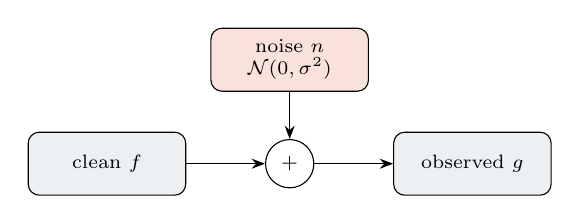
\begin{tikzpicture}[font=\scriptsize,>=Stealth,node distance=4mm and 10mm,
    b/.style={draw,rounded corners,fill=coursePrimary!8,minimum height=8mm,minimum width=20mm,align=center}]
    \node[b] (f){clean $f$};
    \node[circle,draw,right=of f] (plus){$+$};
    \node[b,above=6mm of plus,fill=courseAccent!20] (n){noise $n$\\$\mathcal{N}(0,\sigma^2)$};
    \node[b,right=of plus] (g){observed $g$};
    \draw[->](f)--(plus);\draw[->](n)--(plus);\draw[->](plus)--(g);
  \end{tikzpicture}
  \end{center}
  \begin{itemize}
    \item Denoising = estimate $f$ given only $g$. We never see $n$ directly.
    \item Because $n$ is \term{zero-mean}, \emph{averaging} independent samples of the same signal drives $n$ toward $0$ — the whole basis of smoothing filters.
  \end{itemize}
\end{frame}

\begin{frame}{Diagnosing noise}
  \begin{itemize}
    \item Look at a \term{flat} region: Gaussian = a fuzzy spread; salt-pepper = isolated black/white specks.
    \item The histogram of a flat patch: Gaussian widens the peak into a bell; impulse adds spikes at 0 and 255.
    \item Match the filter to what you see — using the wrong one wastes detail or fails to clean.
  \end{itemize}
  \begin{badbox}
    Averaging (Gaussian blur) barely touches salt-and-pepper — it just spreads each speck into a gray smudge.
  \end{badbox}
\end{frame}

\begin{frame}{Histogram of a flat patch}
  \begin{columns}[T]
    \begin{column}{0.5\textwidth}\begin{center}
    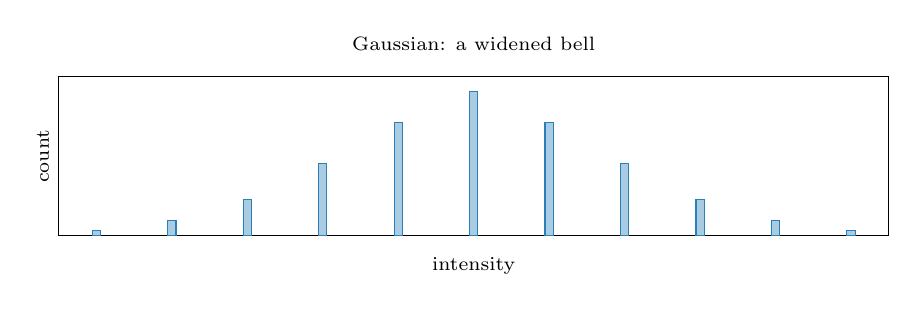
\begin{tikzpicture}
      \begin{axis}[width=\linewidth,height=3.6cm,ybar,bar width=3pt,
        title={\scriptsize Gaussian: a widened bell},
        xlabel={\scriptsize intensity},ylabel={\scriptsize count},
        xtick=\empty,ytick=\empty,ymin=0,enlarge x limits=0.05]
        \addplot[draw=courseInfo,fill=courseInfo!40] coordinates {
          (1,1)(2,3)(3,7)(4,14)(5,22)(6,28)(7,22)(8,14)(9,7)(10,3)(11,1)};
      \end{axis}
    \end{tikzpicture}
    \end{center}\end{column}
    \begin{column}{0.5\textwidth}\begin{center}
    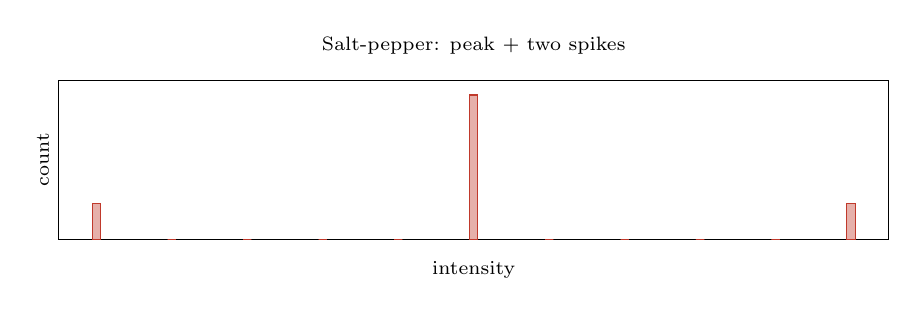
\begin{tikzpicture}
      \begin{axis}[width=\linewidth,height=3.6cm,ybar,bar width=3pt,
        title={\scriptsize Salt-pepper: peak + two spikes},
        xlabel={\scriptsize intensity},ylabel={\scriptsize count},
        xtick=\empty,ytick=\empty,ymin=0,enlarge x limits=0.05]
        \addplot[draw=courseBad,fill=courseBad!40] coordinates {
          (1,10)(2,0)(3,0)(4,0)(5,0)(6,40)(7,0)(8,0)(9,0)(10,0)(11,10)};
      \end{axis}
    \end{tikzpicture}
    \end{center}\end{column}
  \end{columns}
  \keyidea{One glance at the flat-patch histogram tells you which family you are fighting — bell vs spikes.}
\end{frame}

\begin{frame}{Worked: reading noise off a patch}
  A supposedly uniform gray wall ($\approx120$) measured as:
  \begin{center}\pixelgrid{ {118,122,255,119,121}, {120,0,121,123,118}, {119,124,120,255,122} }\end{center}
  \begin{itemize}
    \item Most values cluster near 120 with a $\pm 4$ spread $\rightarrow$ a \term{Gaussian} component.
    \item Three values are \textbf{0} or \textbf{255} — nowhere near 120 $\rightarrow$ \term{impulse} contamination.
    \item Diagnosis: \emph{both} noises present $\Rightarrow$ median first (kill specks), then a light average.
  \end{itemize}
\end{frame}

% ==================================================================
\section{Averaging \& Gaussian smoothing}
% ==================================================================

\begin{frame}{Removing Gaussian noise by averaging}
  \begin{columns}[T]
    \begin{column}{0.5\textwidth}\begin{center}
      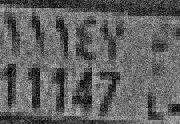
\includegraphics[width=0.9\linewidth]{../assets/gaussian_noise.png}\\{\scriptsize noisy}
    \end{center}\end{column}
    \begin{column}{0.5\textwidth}\begin{center}
      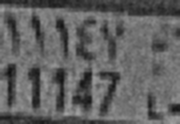
\includegraphics[width=0.9\linewidth]{../assets/gauss_denoise_gauss.png}\\{\scriptsize Gaussian blur}
    \end{center}\end{column}
  \end{columns}
  \vspace{3pt}
  \begin{itemize}
    \item Averaging a neighbourhood sums many noisy samples of (nearly) the same signal — the noise partly cancels.
    \item Cost: real edges also get averaged, so the result is smoother \emph{and} softer. (Session 2 fixes this.)
  \end{itemize}
\end{frame}

\begin{frame}{Why averaging works: the $\sqrt{N}$ rule}
  \begin{mathbox}
    Average $N$ independent samples of variance $\sigma^2$:
    $\quad\mathrm{Var}\!\left(\tfrac1N\sum n_i\right)=\dfrac{\sigma^2}{N}
    \;\Rightarrow\; \sigma_{\text{out}}=\dfrac{\sigma}{\sqrt{N}}.$
  \end{mathbox}
  \begin{itemize}
    \item A $3\times3$ mean averages $N=9$ pixels $\rightarrow$ noise drops by $\sqrt{9}=3\times$.
    \item A $5\times5$ mean ($N=25$) $\rightarrow$ $5\times$ less noise, but $5\times$ more blur too.
    \item Diminishing returns: to halve noise again you must \emph{quadruple} the window.
  \end{itemize}
  \keyidea{Bigger window = less noise \emph{and} more blur. The window size \emph{is} the trade-off knob.}
\end{frame}

\begin{frame}{Mean filter vs Gaussian filter}
  \begin{columns}[T]
    \begin{column}{0.5\textwidth}
    \begin{center}{\scriptsize box (mean) kernel}\\[2pt]
      $\dfrac{1}{9}\begin{bmatrix}1&1&1\\1&1&1\\1&1&1\end{bmatrix}$
    \end{center}
    All neighbours weighted equally $\rightarrow$ slightly boxy, can ring.
    \end{column}
    \begin{column}{0.5\textwidth}
    \begin{center}{\scriptsize Gaussian kernel ($\sigma\!\approx\!1$)}\\[2pt]
      $\dfrac{1}{16}\begin{bmatrix}1&2&1\\2&4&2\\1&2&1\end{bmatrix}$
    \end{center}
    Centre-weighted $\rightarrow$ smoother, no boxiness, separable \& fast.
    \end{column}
  \end{columns}
  \vspace{4pt}
  \begin{goodbox}
    Both kernels sum to 1 (normalized) so the average brightness is preserved. Prefer the Gaussian: it is isotropic and separable.
  \end{goodbox}
\end{frame}

\begin{frame}{Worked: mean of a $3\times3$ patch}
  Noisy patch around a flat gray value:
  \begin{center}\pixelgrid{ {121,118,122}, {119,255,120}, {123,117,120} }\end{center}
  \begin{itemize}
    \item \term{Mean} $=\frac{1}{9}(121{+}118{+}122{+}119{+}255{+}120{+}123{+}117{+}120)=\frac{1215}{9}=135$.
    \item The single \textbf{255} outlier dragged the estimate from $\sim120$ up to \textbf{135}.
    \item Averaging \emph{smeared} the impulse into every output near it instead of removing it.
  \end{itemize}
  \begin{badbox}
    One impulse pixel poisons the whole window under averaging. Remember this when we compare with the median.
  \end{badbox}
\end{frame}

\begin{frame}{Choosing $\sigma$ and window size}
  \begin{itemize}
    \item Rule of thumb: kernel radius $\approx 3\sigma$ so the tail is negligible; e.g. $\sigma=1 \Rightarrow$ a $7\times7$ ($r=3$) window.
    \item Larger $\sigma$ = stronger smoothing = more noise gone \emph{and} more detail gone.
    \item Pick $\sigma$ from the \emph{feature} you must keep: it should be smaller than the thinnest stroke of a digit.
  \end{itemize}
  \begin{infobox}
    For meter digits a few pixels wide, $\sigma\!=\!1$ ($3\times3$) is usually the ceiling — beyond it the strokes fuse.
  \end{infobox}
\end{frame}

\begin{frame}{Boundary handling}
  \begin{itemize}
    \item The window falls off the image edge — what fills the missing neighbours?
    \item \term{Replicate} (clamp) the edge pixel, \term{reflect} the image, \term{wrap} around, or \term{zero}-pad.
    \item Zero-padding darkens borders (a black frame bleeds in); \emph{reflect} is the safest default.
  \end{itemize}
  \begin{center}
  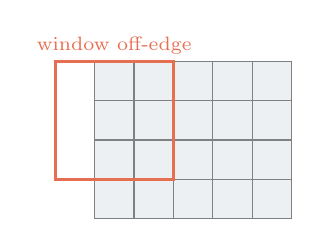
\begin{tikzpicture}[font=\scriptsize,scale=0.5]
    \foreach \x in {0,...,4}\foreach \y in {0,...,3}
      \draw[gray,fill=coursePrimary!8] (\x,\y) rectangle ++(1,1);
    \draw[courseAccent,very thick] (-1,1) rectangle (2,4);
    \node[courseAccent] at (0.5,4.4) {window off-edge};
  \end{tikzpicture}
  \end{center}
\end{frame}

% ==================================================================
\section{The median filter}
% ==================================================================

\begin{frame}{Removing salt-and-pepper — median wins}
  \begin{columns}[T]
    \begin{column}{0.33\textwidth}\begin{center}
      
\includegraphics[width=\linewidth]{../assets/sp_noise.png}\\{\scriptsize noisy}
    \end{center}\end{column}
    \begin{column}{0.33\textwidth}\begin{center}
      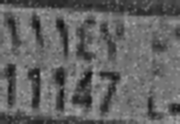
\includegraphics[width=\linewidth]{../assets/sp_denoise_gauss.png}\\{\scriptsize Gaussian (bad)}
    \end{center}\end{column}
    \begin{column}{0.33\textwidth}\begin{center}
      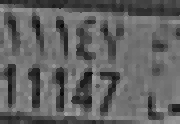
\includegraphics[width=\linewidth]{../assets/sp_denoise_median.png}\\{\scriptsize median (great)}
    \end{center}\end{column}
  \end{columns}
  \vspace{3pt}
  \keyidea{The median ignores outliers: a speck of 255 among 100s doesn't move the median.
  This is why median crushes impulse noise while keeping edges.}
\end{frame}

\begin{frame}{Why median beats averaging for impulse noise}
  \begin{itemize}
    \item Mean of $\{100,100,100,255\}$ = 164 — the outlier drags it up.
    \item Median of the same = 100 — the outlier is ignored entirely.
    \item Averaging \emph{spreads} an impulse; median \emph{deletes} it. Match filter to noise.
  \end{itemize}
  \begin{mathbox}
    The median minimizes $\sum_i |x_i - m|$ (robust); the mean minimizes $\sum_i (x_i-m)^2$, so a single far outlier dominates it.
  \end{mathbox}
\end{frame}

\begin{frame}{Worked: median of the same patch}
  Same noisy patch as before:
  \begin{center}\pixelgrid{ {121,118,122}, {119,255,120}, {123,117,120} }\end{center}
  \begin{enumerate}
    \item Sort the 9 values: $117,118,119,120,\mathbf{120},121,122,123,255$.
    \item The 5th (middle) value is the \term{median} $=\mathbf{120}$.
    \item The \textbf{255} sits harmlessly at the end of the list — it never reaches the middle.
  \end{enumerate}
  \begin{goodbox}
    Median gave \textbf{120} (the true gray); the mean gave \textbf{135}. Same data, right filter.
  \end{goodbox}
\end{frame}

\begin{frame}{Median mechanics: sort \& pick the middle}
  \begin{center}
  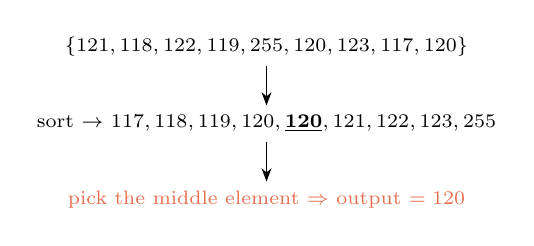
\begin{tikzpicture}[font=\scriptsize,>=Stealth,node distance=6mm]
    \node (a) {$\{121,118,122,119,255,120,123,117,120\}$};
    \node[below=5mm of a] (b) {sort $\rightarrow$ $117,118,119,120,\underline{\mathbf{120}},121,122,123,255$};
    \node[below=5mm of b,courseAccent] (c) {pick the middle element $\Rightarrow$ output $=120$};
    \draw[->](a)--(b);\draw[->](b)--(c);
  \end{tikzpicture}
  \end{center}
  \begin{itemize}
    \item It is \term{non-linear}: you cannot write it as a convolution kernel.
    \item It preserves \term{step edges} exactly (the middle value is a real pixel, never a blend).
    \item Cost: sorting each window; use small windows ($3\times3$, $5\times5$) or a running histogram.
  \end{itemize}
\end{frame}

\begin{frame}{A quick reference of noise $\rightarrow$ filter}
  \begin{center}
  \begin{tabular}{@{}lll@{}}
    \toprule
    \textbf{Noise} & \textbf{Looks like} & \textbf{Best filter} \\
    \midrule
    Gaussian & fuzzy grain everywhere & Gaussian / NLM \\
    Salt-and-pepper & isolated black/white dots & median \\
    Poisson (shot) & grain, worse in dark & NLM / variance-stabilize \\
    Periodic & repeating wave/pattern & frequency-domain (Week 6) \\
    \bottomrule
  \end{tabular}
  \end{center}
  \keyidea{Periodic noise is invisible to spatial filters — you remove it in the frequency domain (Week 6).}
\end{frame}

\begin{frame}[fragile]{The two core filters in code}
\begin{lstlisting}[language=Python]
import cv2
gauss  = cv2.GaussianBlur(noisy, (5,5), 0)   # grain / Gaussian noise
median = cv2.medianBlur(noisy, 3)            # salt-and-pepper specks

# diagnose first: peek at a flat patch
patch = noisy[y:y+15, x:x+15]
print(patch.std())   # wide spread -> Gaussian; 0/255 spikes -> impulse
\end{lstlisting}
  \begin{infobox}
    Try median first for specks; averaging/Gaussian for grain. Measure, don't guess — Session 2 shows how (PSNR/SSIM).
  \end{infobox}
\end{frame}

\begin{frame}{Common pitfalls}
  \begin{badbox}[Wrong filter for the noise]
    Gaussian blur on salt-and-pepper just smears each speck into a gray blob — the dots survive.
  \end{badbox}
  \begin{badbox}[Even-sized / huge windows]
    Even windows have no single middle; oversized windows erase thin digit strokes. Use small, odd windows.
  \end{badbox}
  \begin{badbox}[Skipping the diagnosis]
    Applying a filter before looking at a flat patch wastes detail. Diagnose, then choose.
  \end{badbox}
\end{frame}

% ==================================================================
\section{In-class exercise}
% ==================================================================

\begin{frame}{\faPen~In-class exercise (10 min)}
  \begin{infobox}[Pick the filter — and defend it]
  \end{infobox}
  For each situation, which filter and why?
  \begin{enumerate}
    \item A scanned meter with random black/white dots.
    \item A low-light phone photo with fine grain everywhere.
    \item A patch reads $\{119,121,0,120,255,118,122,120,121\}$ — compute both the mean and the median.
    \item You have five still shots of the \emph{same} meter. What is the cheapest way to cut the grain?
  \end{enumerate}
\end{frame}

\begin{frame}{\faPen~Debrief}
  \begin{itemize}
    \item (1) Salt-and-pepper $\rightarrow$ \term{median}. (2) Gaussian grain $\rightarrow$ Gaussian/mean.
    \item (3) Mean $=\frac{996}{9}\approx111$ (pulled by 0 and 255); median (sorted middle) $=120$ — the true value.
    \item (4) \term{Average the five frames}: noise falls by $\sqrt{5}\approx2.2\times$ with \emph{zero} blur (more in Session 2).
  \end{itemize}
  \keyidea{``Denoise'' isn't one button — it's choosing the model that matches the noise.}
\end{frame}

% ==================================================================
\section{Wrap-up}
% ==================================================================

\begin{frame}{What you should now be able to do}
  \begin{itemize}
    \item Name the physical origin of Gaussian, impulse, and Poisson noise.
    \item Diagnose noise from a flat patch and its histogram.
    \item Apply averaging/Gaussian for grain and median for specks — and justify each with a worked example.
    \item Reason quantitatively about the $\sqrt{N}$ noise reduction and the noise-vs-blur trade-off.
  \end{itemize}
\end{frame}

\begin{frame}{Next session}
  \begin{alertblock}{Session 2 — Edge-preserving restoration \& measuring quality}
    \begin{itemize}
      \item Filters that smooth flats \emph{without} blurring edges: \term{bilateral} \& \term{non-local means}.
      \item \term{Adaptive} \& order-statistic filters; \term{temporal} multi-frame averaging.
      \item Deblurring \& the PSF; and how to \emph{measure} restoration with \term{PSNR}/\term{SSIM}.
      \item Then the week's deliverable. (No deliverable yet — just come with your worked exercise.)
    \end{itemize}
  \end{alertblock}
\end{frame}

\begin{frame}[standout]
  Diagnose, then denoise.\\[4pt]
  \normalsize Averaging for grain, median for specks — matched to the noise you actually see.
\end{frame}

\end{document}
